\section{小規模問題での厳密な解析}\label{sec:small}

\subsection{設定}

18〜24 頂点の問題を 30 個作った．種類は，ランダム 3 正則グラフ（重み 1），平均次数 4 の Erdős--Rényi グラフに重み $\pm1$ をつけたもの，$4\times5$・$4\times6$ の格子に確率 0.6 で対角辺を加えた三角格子（重み 1）を各 10 個である．番号の偶数・奇数で開発用と検証用に 15 個ずつ分け，指標と仮説は開発用だけを見て決め，その文書をコミットしてから検証用を解析した．

小規模問題では，CIM を 1500 ラウンド回すとほぼ必ず最適解を出す（最適率 0.95 以上）．大規模問題では CIM の出力は最適解の手前（G-set で最適値との差 0.3〜3\%）にあるので，同じ状況を作るため，増幅の途中の 512 ラウンドで止めた CIM を 1024 回実行し，異なる非最適解を候補とした．1 問題（$\pm1$ 重みの 1 つ）は CIM が常に最適解を出したので除き，29 問題で計 8647 個の候補を得た．各候補に SA（開始温度 0.5，終了温度 0.01）を 256 回かけ，3・10・30 掃引で最適値に到達した割合をラベルとした．候補が 5 個以上ある（問題，初期カット値）の層で比べた．

\subsection{結果}

図\ref{fig:small}に，10 掃引のラベルに対する層内の Kendall $\tau$ を示す．

\begin{figure}[t]
\centering
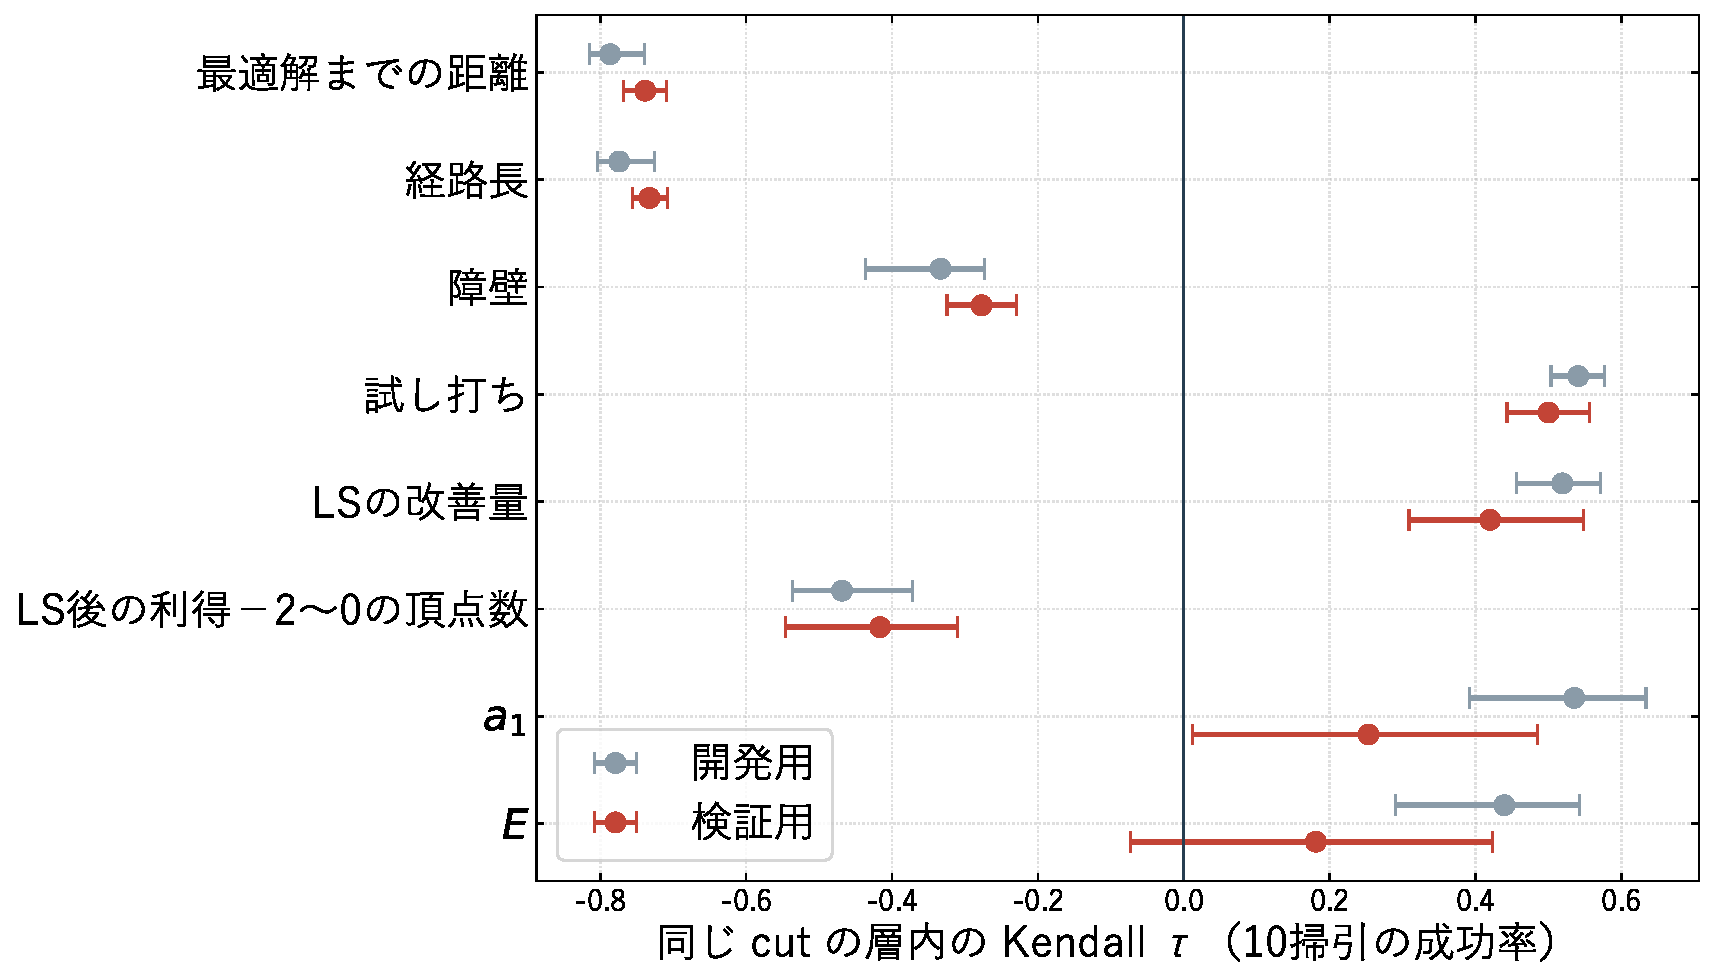
\includegraphics[width=0.72\linewidth]{fig_small_tau.pdf}
\caption{小規模問題で，同じ初期カット値の候補の中での，指標と SA の最適到達率（10 掃引）の Kendall $\tau$．灰色は開発用 14 問題，赤は検証用 15 問題．区間は問題を単位にしたブートストラップの 95\% 区間．}\label{fig:small}
\end{figure}

\paragraph{種の価値はほぼ最適解までの距離で決まる.} 厳密量のうち，最適解までのハミング距離（検証用 $\tau=-0.74$，偏 $R^2=0.65$）と経路長（$-0.73$，$0.60$）が最も強く，両者はほぼ同じ量だった（互いの $\tau=0.97$）．障壁は弱かった（$-0.28$，$0.26$）．多くの候補はカット値を下げずに最適解へ行け（障壁 $>0$ の候補は問題ごとに 0〜29\%），後段の SA にとっての難しさは「越えるべき山の高さ」より「進むべき距離」で決まっていた．

\paragraph{局所的な指標と試し打ちは安定して効く.} 試し打ち（1 掃引の SA を 8 回，$\tau=0.50$），LS の改善量（$0.42$），LS 後に利得が $-2$〜$0$ の頂点数（$-0.42$）は，開発用と検証用で同程度に効いた．試し打ちと LS の改善量は，3 種類の問題のいずれでも区間が 0 を含まなかった．

\paragraph{固有ベクトル指標は問題によって効き方が違う.} 開発用では $a_1$ が強かった（$\tau=0.54$）が，検証用では $0.25$（[$0.01$, $0.49$]）に下がった．事前登録の $E$ は検証用で確認できなかった（$0.18$，[$-0.07$, $0.42$]）．種類別に見ると，3 正則グラフと三角格子では開発用で $\tau=0.49$〜$0.61$ と強いが，$\pm1$ 重みのグラフではほぼ効かない（開発用 $0.20$，検証用 $0.02$）．また，検証用でも問題ごとのばらつきが大きく，区間が広い．一方，$a_1$ は最適解までの距離と対応していた（検証用 $\tau=-0.30$，[$-0.56$, $-0.04$]）．$u_1$ の符号パターンに近い候補は最適解にも近い傾向があり，固有ベクトル指標が効くときの仕組みは「最適解への近さの粗い代理」と解釈できる．

\paragraph{予算への依存.} 3 掃引では試し打ちと局所的な指標の偏 $R^2$ が大きく，30 掃引では最適解までの距離の偏 $R^2$ が大きくなった（開発用で 3・10・30 掃引の順に 0.59，0.70，0.74）．短い予算では「すぐ取れる改善」が，長い予算では大域的な位置が効くという傾向は，G22 で $E$ が長い予算でだけ効いたこと（表\ref{tab:prereg}）と整合する．
